\documentclass[border=4pt]{standalone}
\usepackage{tikz}
\usetikzlibrary{positioning, arrows.meta, shapes.geometric, calc, fit, backgrounds}
\usepackage{amsmath,amssymb}
\begin{document}
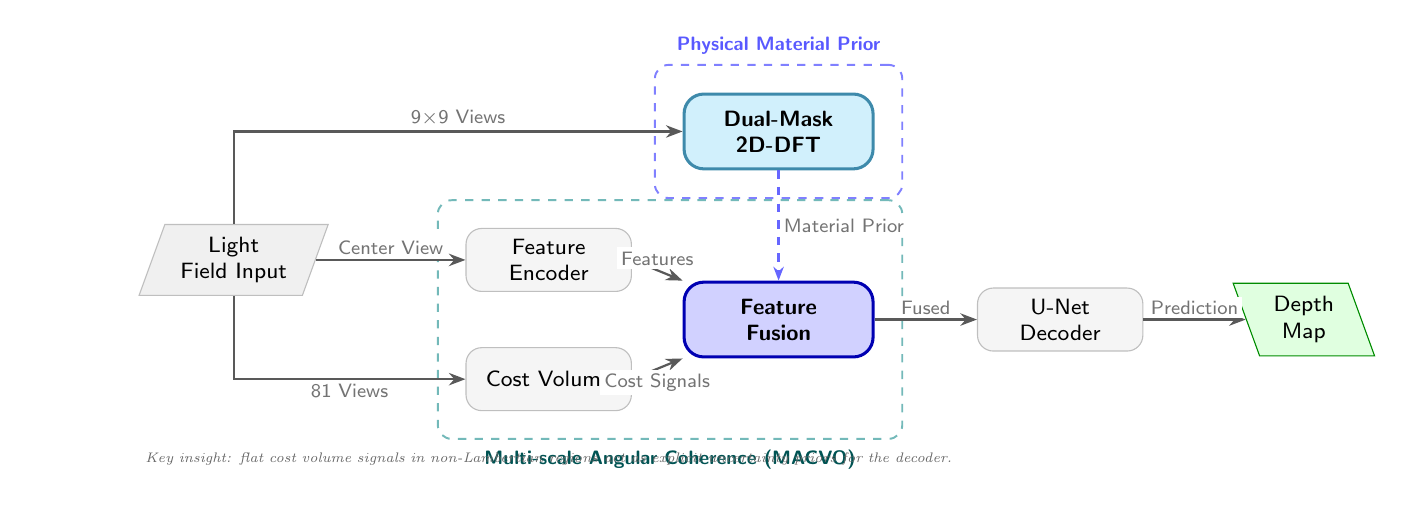
\begin{tikzpicture}[
  >=Stealth,
  input/.style={draw, trapezium, trapezium left angle=70, trapezium right angle=110,
                minimum width=1.8cm, minimum height=0.9cm,
                fill=gray!12, draw=gray!50, align=center, font=\sffamily\footnotesize},
  module/.style={draw, rounded corners=2mm, minimum width=2.1cm, minimum height=0.8cm,
                 fill=gray!8, draw=gray!50, align=center, font=\sffamily\footnotesize},
  innov/.style={draw, rounded corners=2.5mm, minimum width=2.4cm, minimum height=0.95cm,
                fill=blue!18, draw=blue!70!black, line width=1.1pt, align=center,
                font=\sffamily\footnotesize\bfseries},
  innov2/.style={draw, rounded corners=2.5mm, minimum width=2.4cm, minimum height=0.95cm,
                 fill=cyan!18, draw=cyan!65!black, line width=1.1pt, align=center,
                 font=\sffamily\footnotesize\bfseries},
  output/.style={draw, trapezium, trapezium left angle=110, trapezium right angle=70,
                 minimum width=1.8cm, minimum height=0.9cm,
                 fill=green!12, draw=green!55!black, align=center, font=\sffamily\footnotesize},
  arr/.style={-{Stealth[length=6pt]}, thick, color=black!65},
  arrd/.style={-{Stealth[length=5pt]}, dashed, color=blue!60, line width=0.9pt},
  lbl/.style={font=\sffamily\scriptsize, text=black!55, fill=white, inner sep=1.5pt},
  glbl/.style={font=\sffamily\scriptsize\bfseries},
  gbox/.style={draw=#1, dashed, rounded corners=5pt, inner sep=10pt, line width=0.7pt},
]

% --- Input ---
\node[input] (m1) {Light\\Field Input};

% --- MACVO branch modules ---
\node[module, right=1.9cm of m1] (m3) {Feature\\Encoder};
\node[module, below=0.7cm of m3] (m4) {Cost Volume};

% --- Fusion (innovation) ---
\coordinate (mid34) at ($(m3)!0.5!(m4)$);
\node[innov, right=1.7cm of mid34] (m5) {Feature\\Fusion};

% --- Physical Prior (innovation, above) ---
\node[innov2, above=1.4cm of m5] (m2) {Dual-Mask\\2D-DFT};

% --- Decoder ---
\node[module, right=1.3cm of m5] (m6) {U-Net\\Decoder};

% --- Output ---
\node[output, right=1.3cm of m6] (m7) {Depth\\Map};

% --- Arrows (main flow) ---
\draw[arr] (m1.north) |- node[lbl, near end, above] {9$\times$9 Views} (m2.west);
\draw[arr] (m1.east) -- node[lbl, above] {Center View} (m3.west);
\draw[arr] (m1.south) |- node[lbl, near end, below] {81 Views} (m4.west);

\draw[arrd] (m2.south) -- node[lbl, right] {Material Prior} (m5.north);
\draw[arr] (m3.east) -- node[lbl, above] {Features} (m5.north west);
\draw[arr] (m4.east) -- node[lbl, below] {Cost Signals} (m5.south west);

\draw[arr] (m5.east) -- node[lbl, above] {Fused} (m6.west);
\draw[arr] (m6.east) -- node[lbl, above] {Prediction} (m7.west);

% --- Group boxes (background) ---
\begin{scope}[on background layer]
  \node[gbox=blue!50, fit=(m2),
        label={[glbl, text=blue!65]above:Physical Material Prior}] {};
  \node[gbox=teal!55, fit=(m3)(m4)(m5),
        label={[glbl, text=teal!65!black]below:Multi-scale Angular Coherence (MACVO)}] {};
\end{scope}

% --- Key annotation ---
\node[font=\tiny\itshape, text=black!60, align=center, text width=13cm,
      below=0.4cm of m4] (note)
  {Key insight: flat cost volume signals in non-Lambertian regions act as explicit uncertainty priors for the decoder.};

\end{tikzpicture}
\end{document}